\section{解析と結果}

\subsection{光量の評価}
今回の解析では、発生光子数ではなく何個のMPPCに光子が入ったかを表すMultiplicityで光量の評価を行った。

\begin{figure}[htbp]
  \centering
  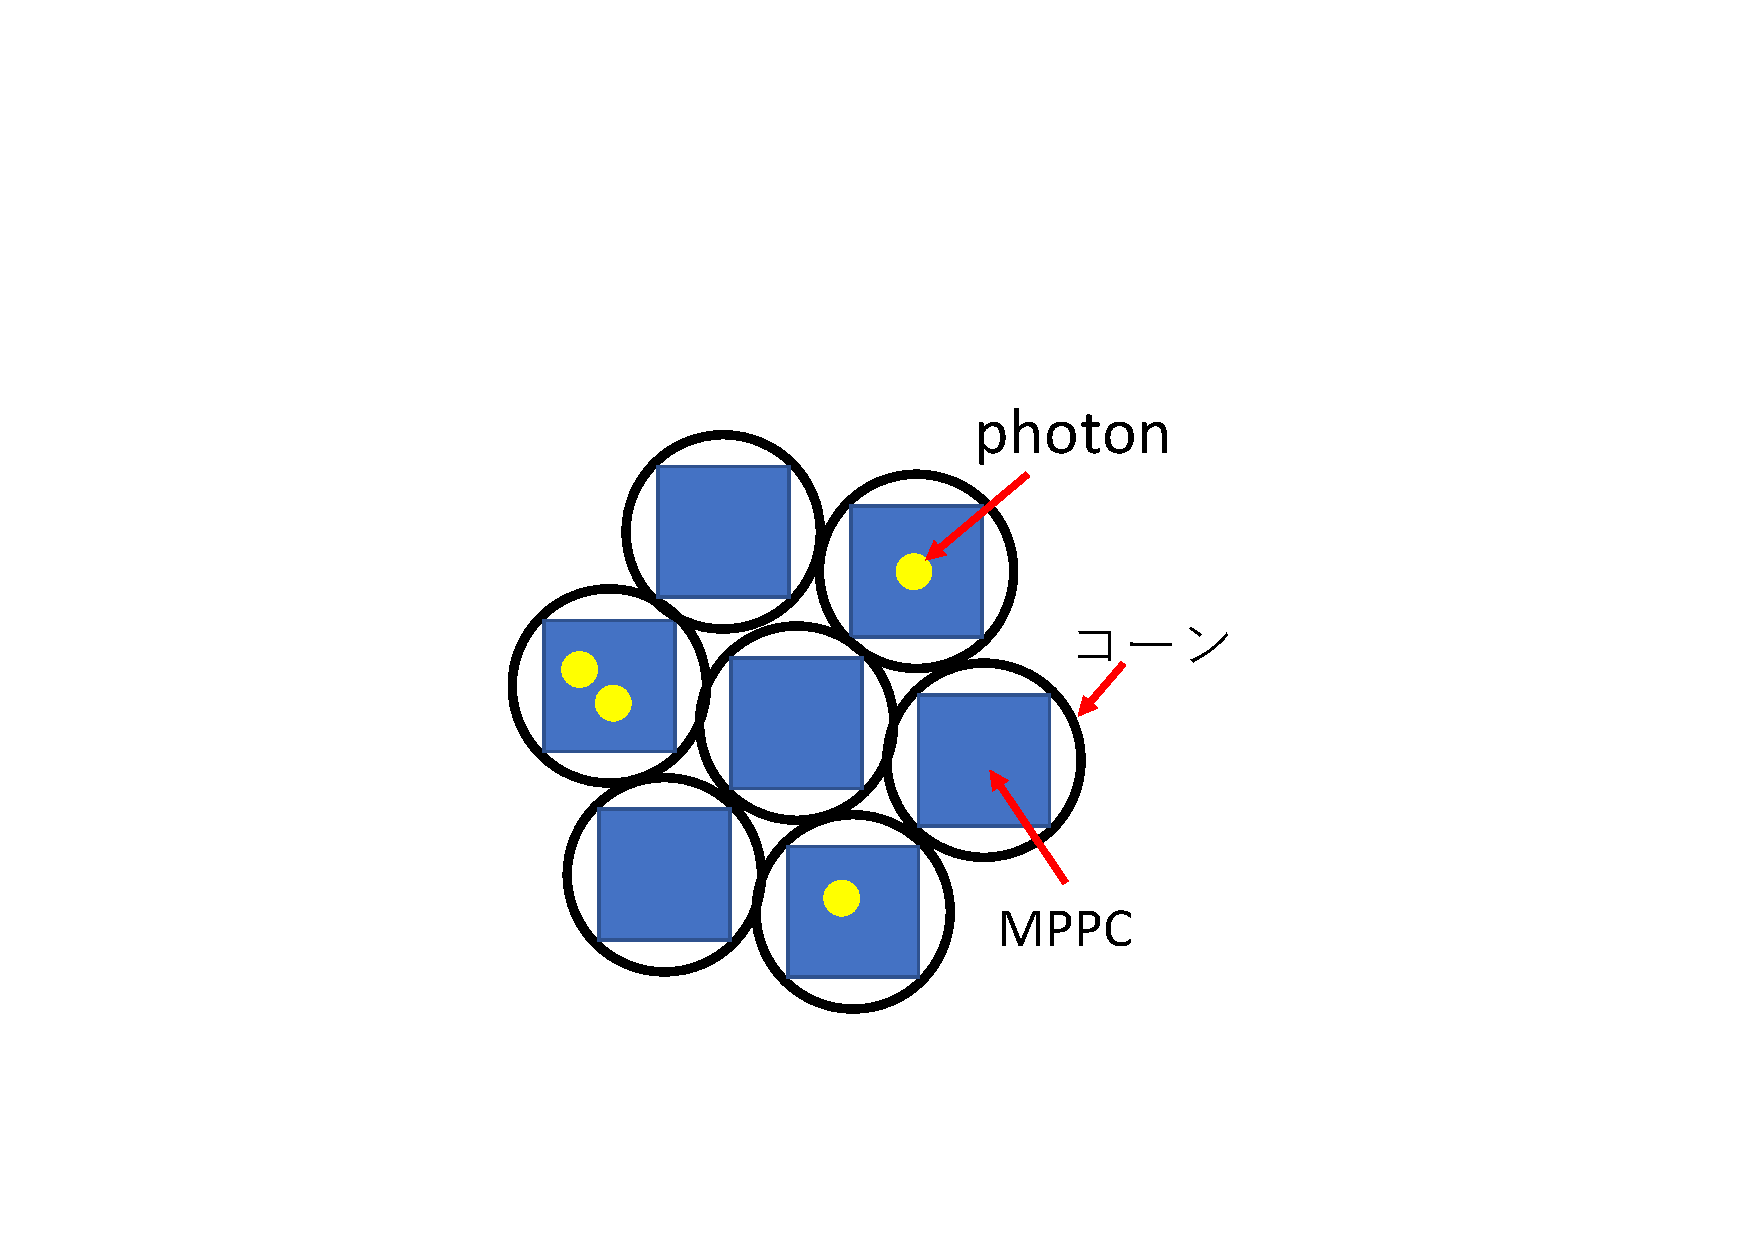
\includegraphics[width=10cm]{images/chapter3/Multiplicity.pdf}
  \caption{Multiplicityの概念図。MultiplicityはPhotonを検出したMPPCの数であるため、この図の場合光子数は4だがMultiplicityは3となる。}
  \label{fig:Multiplicity}
\end{figure}

\subsection{暗電流の評価}